\documentclass[../../../main.tex]{subfiles}
\begin{document}

%%%%%%%%%%%%%%%%%%%%%%%%%%%%%%%%%%%%%%%%%
%%%%%%%%%%%%%%%%%%%%%%%%%%%%%%%%%%%%%%%%%
%%%%%%%%%%%%%%%%%%%%%%%%%%%%%%%%%%%%%%%%%
\chapter{Type II Errors}


Type II Errors are exactly the opposite of Type I Errors. A Type I Error occurs when you mistakenly \emph{reject} a null hypothesis, whereas a Type II Error occurs when you mistakenly \emph{accept} a null hypothesis.


%%%%%%%%%%%%%%%%%%%%%%%%%%%%%%%%%%%%%%%%%
%%%%%%%%%%%%%%%%%%%%%%%%%%%%%%%%%%%%%%%%%
\section{No Type II Error}

How does a Type II Error happen? Let us first consider a case where it cannot happen. Then we will see how it can happen. 

So first, consider the following. Suppose we have a hypothesized population mean $\HypPopMean/$ set to 55K (as before), and suppose that we set $\alpha$ to 5\% of that sampling distribution, like this:

\begin{center}
  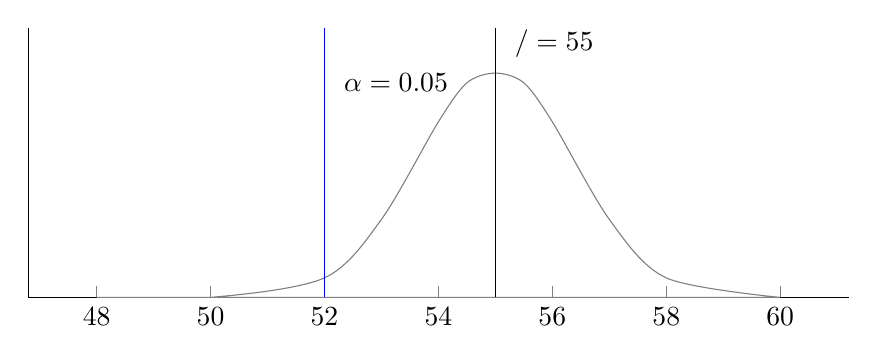
\begin{tikzpicture}
    \begin{axis}[
      axis lines*=left,
      ytick=\empty,
      height=5cm,
      width=12cm,
      enlarge y limits={value=0.2,upper},
      ]

      \addplot[smooth, color=gray, domain=45:65] 
        coordinates{
          (48, 0)
          (50, 0) (52, 0.5) (53, 2) (54, 4.5) (54.5, 5.5)
          (55, 5.75)
          (55.5, 5.5) (56, 4.5) (57, 2) (58, 0.5) (60, 0)} 
        \closedcycle;

      \draw (55, 0) -- (55, 10);
      \node at (55, 6.5) [label=right:{$\HypPopMean/ = 55$}] {};

      \draw[color=blue] (52, 0) -- (52, 10);
      \node at (52, 5.5) [label=right:{$\alpha = 0.05$}] {};

    \end{axis}
  \end{tikzpicture}
\end{center}

\noindent
Now suppose that, as an all-seeing God or Oracle, we know that the true population mean is much lower, at 43K:

\begin{center}
  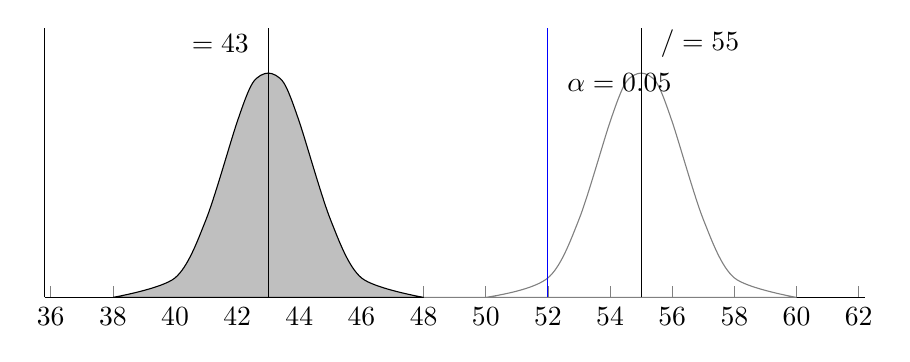
\begin{tikzpicture}
    \begin{axis}[
      axis lines*=left,
      ytick=\empty,
      height=5cm,
      width=12cm,
      enlarge y limits={value=0.2,upper},
      ]

      \addplot[smooth, color=gray, domain=45:65] 
        coordinates{
          (48, 0)
          (50, 0) (52, 0.5) (53, 2) (54, 4.5) (54.5, 5.5)
          (55, 5.75)
          (55.5, 5.5) (56, 4.5) (57, 2) (58, 0.5) (60, 0)} 
        \closedcycle;

      \draw (55, 0) -- (55, 10);
      \node at (55, 6.5) [label=right:{$\HypPopMean/ = 55$}] {};

      \addplot[smooth, fill=lightgray, domain=45:65] 
        coordinates{
          (38, 0) (40, 0.5) (41, 2) (42, 4.5) (42.5, 5.5)
          (43, 5.75)
          (43.5, 5.5) (44, 4.5) (45, 2) (46, 0.5) (48, 0)} 
        \closedcycle;

      \draw (43, 0) -- (43, 10);
      \node at (43, 6.5) [label=left:{$\populationmean = 43$}] {};

      \draw[color=blue] (52, 0) -- (52, 10);
      \node at (52, 5.5) [label=right:{$\alpha = 0.05$}] {};

    \end{axis}
  \end{tikzpicture}
\end{center}

\noindent
If we take a sample, that sample will have a mean somewhere in the grey area, since our sample comes from the real population. Since that sample mean is far below $\alpha$, we will reject the null hypothesis. In this case, we will in fact do it correctly, since the true population mean (at 43K) really is well below the hypothesized population mean (at 55K).

Can we mistakenly accept the null hypothesis in this scenario? No, it is impossible. Since the true population mean is so far below the hypothesized population mean, any sample we could possibly take from the true population will be well below the hypothesized sampling mean.


%%%%%%%%%%%%%%%%%%%%%%%%%%%%%%%%%%%%%%%%%
%%%%%%%%%%%%%%%%%%%%%%%%%%%%%%%%%%%%%%%%%
\section{Some Type II Error}

Now let us slide the true population mean over to the right, until we have some overlap. For example, suppose we slide the true population mean over until it's at 50K:

\begin{center}
  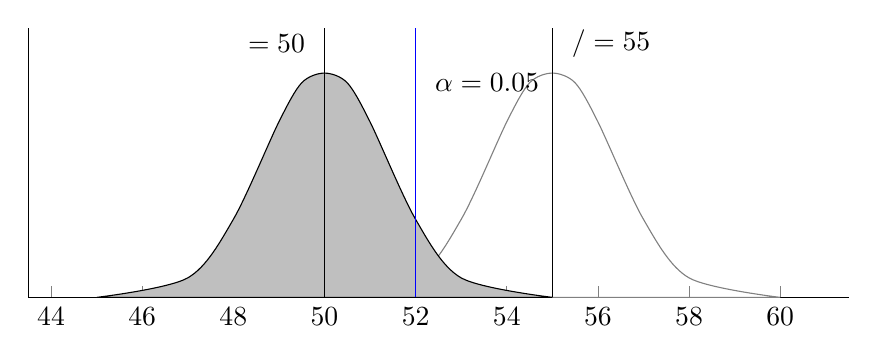
\begin{tikzpicture}
    \begin{axis}[
      axis lines*=left,
      ytick=\empty,
      height=5cm,
      width=12cm,
      enlarge y limits={value=0.2,upper},
      ]

      \addplot[smooth, color=gray, domain=45:65] 
        coordinates{
          (48, 0)
          (50, 0) (52, 0.5) (53, 2) (54, 4.5) (54.5, 5.5)
          (55, 5.75)
          (55.5, 5.5) (56, 4.5) (57, 2) (58, 0.5) (60, 0)} 
        \closedcycle;

      \draw (55, 0) -- (55, 10);
      \node at (55, 6.5) [label=right:{$\HypPopMean/ = 55$}] {};

      \addplot[smooth, fill=lightgray, domain=45:65] 
        coordinates{
          (45, 0) (47, 0.5) (48, 2) (49, 4.5) (49.5, 5.5)
          (50, 5.75)
          (50.5, 5.5) (51, 4.5) (52, 2) (53, 0.5) (55, 0)} 
        \closedcycle;

      \draw (50, 0) -- (50, 10);
      \node at (50, 6.5) [label=left:{$\populationmean = 50$}] {};

      \draw[color=blue] (52, 0) -- (52, 10);
      \node at (52, 5.5) [label=right:{$\alpha = 0.05$}] {};

    \end{axis}
  \end{tikzpicture}
\end{center}

\noindent
At this point, the two sampling distributions overlap. So, suppose that we take a sample, and it has a mean of 53:

\begin{center}
  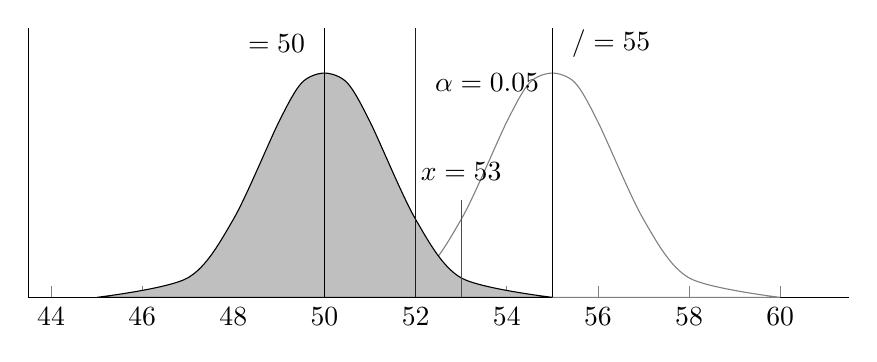
\begin{tikzpicture}
    \begin{axis}[
      axis lines*=left,
      ytick=\empty,
      height=5cm,
      width=12cm,
      enlarge y limits={value=0.2,upper},
      ]

      \addplot[smooth, color=gray, domain=45:65] 
        coordinates{
          (48, 0)
          (50, 0) (52, 0.5) (53, 2) (54, 4.5) (54.5, 5.5)
          (55, 5.75)
          (55.5, 5.5) (56, 4.5) (57, 2) (58, 0.5) (60, 0)} 
        \closedcycle;

      \draw (55, 0) -- (55, 10);
      \node at (55, 6.5) [label=right:{$\HypPopMean/ = 55$}] {};

      \addplot[smooth, fill=lightgray, domain=45:65] 
        coordinates{
          (45, 0) (47, 0.5) (48, 2) (49, 4.5) (49.5, 5.5)
          (50, 5.75)
          (50.5, 5.5) (51, 4.5) (52, 2) (53, 0.5) (55, 0)} 
        \closedcycle;

      \draw (50, 0) -- (50, 10);
      \node at (50, 6.5) [label=left:{$\populationmean = 50$}] {};

      \draw[color=blue] (52, 0) -- (52, 10);
      \node at (52, 5.5) [label=right:{$\alpha = 0.05$}] {};

      \draw[color=red] (53, 0) -- (53, 2.5);
      \node at (53, 2.5) [label=above:{$\samplemean{x} = 53$}] {};

    \end{axis}
  \end{tikzpicture}
\end{center}

\noindent
As human analysts, we do not know if this sample comes from the sampling distribution centered around 50, or from the one centered around 55. 

What do we do then? Again, we follow our procedure. Our procedure says that we should reject the null hypothesis if your sample mean is below $\alpha$, and accept the null hypothesis if the sample mean is above $\alpha$. In this case, our sample mean is above $\alpha$, so we accept the null hypothesis.

However, once we step into the role of the all-seeing God or Oracle, we can see that the sample came from the true population, which is centered at 50. So we have made a mistake. We accepted the null hypothesis (which claims that the true population is at 55K), even though the true population is 50K, which is lower than 55K. 


%%%%%%%%%%%%%%%%%%%%%%%%%%%%%%%%%%%%%%%%%
%%%%%%%%%%%%%%%%%%%%%%%%%%%%%%%%%%%%%%%%%
\section{The probability of Type II Errors}

As human analysts, again we will never know if we committed a Type II Error or not. The best we can do is calculate the probability of that happening. How do you calculate the probability of a Type II Error?

It is the area of the alternative population sampling distribution that overlaps the non-rejection region of the hypothesized sampling distribution. Here it is in the picture, highlighted:

\begin{center}
  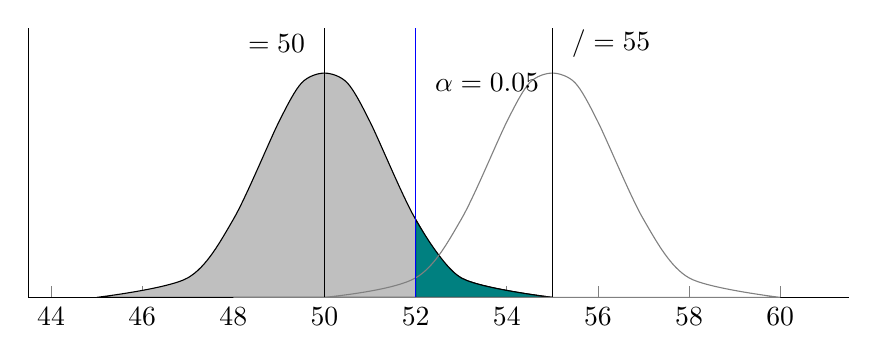
\begin{tikzpicture}
    \begin{axis}[
      axis lines*=left,
      ytick=\empty,
      height=5cm,
      width=12cm,
      enlarge y limits={value=0.2,upper},
      ]

      \addplot[smooth, fill=lightgray, domain=45:65] 
        coordinates{
          (45, 0) (47, 0.5) (48, 2) (49, 4.5) (49.5, 5.5)
          (50, 5.75)
          (50.5, 5.5) (51, 4.5) (52, 2) (53, 0.5) (55, 0)} 
        \closedcycle;

      \addplot[smooth, fill=teal, domain=45:65] 
        coordinates{(52, 2) (53, 0.5) (55, 0)} 
        \closedcycle;

      \addplot[smooth, color=gray, domain=45:65] 
        coordinates{
          (48, 0)
          (50, 0) (52, 0.5) (53, 2) (54, 4.5) (54.5, 5.5)
          (55, 5.75)
          (55.5, 5.5) (56, 4.5) (57, 2) (58, 0.5) (60, 0)} 
        \closedcycle;

      \draw (55, 0) -- (55, 10);
      \node at (55, 6.5) [label=right:{$\HypPopMean/ = 55$}] {};

      \draw (50, 0) -- (50, 10);
      \node at (50, 6.5) [label=left:{$\populationmean = 50$}] {};

      \draw[color=blue] (52, 0) -- (52, 10);
      \node at (52, 5.5) [label=right:{$\alpha = 0.05$}] {};

    \end{axis}
  \end{tikzpicture}
\end{center}

\noindent
So the area of the grey population that overlaps the non-rejection region of the hypothesized population is the probability of making a Type II Error. We call this area \vocab{beta}, or we use the Greek lowercase letter, i.e., $\beta$.

To calculate $\beta$, we find the z-score of the point where $\alpha$ slices through the grey distribution, and then we use that to compute the area of the highlighted portion of the curve, just as we would for any normal curve.


%%%%%%%%%%%%%%%%%%%%%%%%%%%%%%%%%%%%%%%%%
%%%%%%%%%%%%%%%%%%%%%%%%%%%%%%%%%%%%%%%%%
\section{The power test area}

The area of the \emph{rest} of the grey curve is called the \vocab{power test} value, and once we know $\beta$ we can calculate the power test value easily because we can just subtract $\beta$ from the full area of the curve, like this:

\begin{equation*}
  \text{power test} = 1 - \beta
\end{equation*}

\noindent
Here it is, highlighted:

\begin{center}
  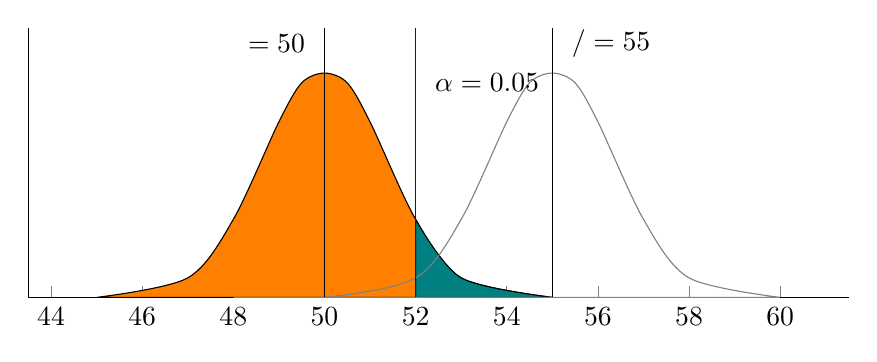
\begin{tikzpicture}
    \begin{axis}[
      axis lines*=left,
      ytick=\empty,
      height=5cm,
      width=12cm,
      enlarge y limits={value=0.2,upper},
      ]

      \addplot[smooth, fill=orange, domain=45:65] 
        coordinates{
          (45, 0) (47, 0.5) (48, 2) (49, 4.5) (49.5, 5.5)
          (50, 5.75)
          (50.5, 5.5) (51, 4.5) (52, 2) (53, 0.5) (55, 0)} 
        \closedcycle;

      \addplot[smooth, fill=teal, domain=45:65] 
        coordinates{(52, 2) (53, 0.5) (55, 0)} 
        \closedcycle;

      \addplot[smooth, color=gray, domain=45:65] 
        coordinates{
          (48, 0)
          (50, 0) (52, 0.5) (53, 2) (54, 4.5) (54.5, 5.5)
          (55, 5.75)
          (55.5, 5.5) (56, 4.5) (57, 2) (58, 0.5) (60, 0)} 
        \closedcycle;

      \draw (55, 0) -- (55, 10);
      \node at (55, 6.5) [label=right:{$\HypPopMean/ = 55$}] {};

      \draw (50, 0) -- (50, 10);
      \node at (50, 6.5) [label=left:{$\populationmean = 50$}] {};

      \draw[color=blue] (52, 0) -- (52, 10);
      \node at (52, 5.5) [label=right:{$\alpha = 0.05$}] {};

    \end{axis}
  \end{tikzpicture}
\end{center}

\noindent
Why do we call this value the ``power test''? Think of that as being a short hand for ``the power \emph{of} the test'' to correctly distinguish between the alternative curve and the hypothesized curve. 


%%%%%%%%%%%%%%%%%%%%%%%%%%%%%%%%%%%%%%%%%
%%%%%%%%%%%%%%%%%%%%%%%%%%%%%%%%%%%%%%%%%
\section{Many alternatives}

We have been speaking about this by comparing the hypothesized sampling distribution with the true sampling distribution, and to do that we occasionally step into the role of an all-seeing God or Oracle so that we can be in a position where we know what the true population mean is. 

But as humans, we never really know where the true sampling distribution is. So really, when we calculate the beta value and the power-test value, we really are thinking of this for any sampling distribution that satisfies the \emph{alternative hypothesis}. 

So, pick any sampling distribution that satisfies the alternative hypothesis $\AltHyp/$, and then you can calculate the $\beta$ and power test values for that alternative sampling distribution, \emph{relative to} the hypothesized sampling distribution proposed by the null hypothesis $\NullHyp/$.

Notice that there as many beta and power-test values as there are sampling distributions that satisfy the alternative hypothesis. In the example of McCallister Logistics that we have been considering here, any population with a mean lower than or equal to 55 will be a population that satisfies the alternative hypothesis. So we can calculate a beta and power-test value for \emph{any} of those alternative populations, relative to the hypothesized population mean of 55K.


%%%%%%%%%%%%%%%%%%%%%%%%%%%%%%%%%%%%%%%%%
%%%%%%%%%%%%%%%%%%%%%%%%%%%%%%%%%%%%%%%%%
\section{A high power test value}

Think about the relationship between $\beta$ and the power test value. Consider a hypothesis test that has a high probability of distinguishing the two curves (i.e., the power test value is high). For such a test, the probability $\beta$ of committing a Type II Error is very low. 

Consider the extreme case where we can't commit a Type II Error at all. Recall the case where the true population was at 43:

\begin{center}
  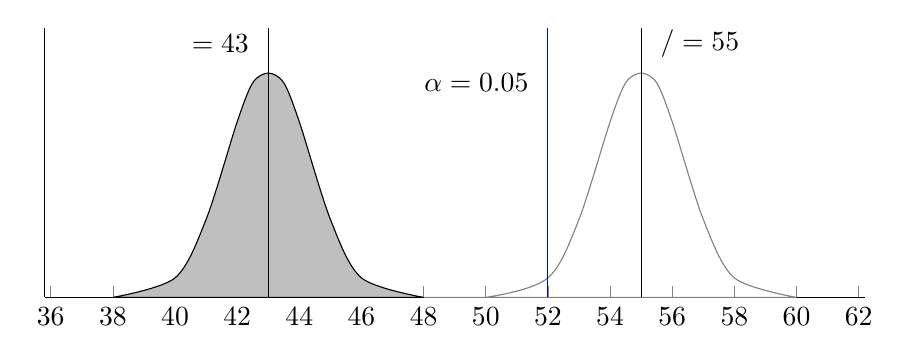
\begin{tikzpicture}
    \begin{axis}[
      axis lines*=left,
      ytick=\empty,
      height=5cm,
      width=12cm,
      enlarge y limits={value=0.2,upper},
      ]

      \addplot[smooth, color=gray, domain=45:65] 
        coordinates{
          (48, 0)
          (50, 0) (52, 0.5) (53, 2) (54, 4.5) (54.5, 5.5)
          (55, 5.75)
          (55.5, 5.5) (56, 4.5) (57, 2) (58, 0.5) (60, 0)} 
        \closedcycle;

      \draw (55, 0) -- (55, 10);
      \node at (55, 6.5) [label=right:{$\HypPopMean/ = 55$}] {};

      \addplot[smooth, fill=lightgray, domain=45:65] 
        coordinates{
          (38, 0) (40, 0.5) (41, 2) (42, 4.5) (42.5, 5.5)
          (43, 5.75)
          (43.5, 5.5) (44, 4.5) (45, 2) (46, 0.5) (48, 0)} 
        \closedcycle;

      \draw (43, 0) -- (43, 10);
      \node at (43, 6.5) [label=left:{$\populationmean = 43$}] {};

      \draw[color=blue] (52, 0) -- (52, 10);
      \node at (52, 5.5) [label=left:{$\alpha = 0.05$}] {};

    \end{axis}
  \end{tikzpicture}
\end{center}

\noindent
Let's highlight the power test area. There is no $\beta$ area on the grey curve here, because the curve doesn't cross over $\alpha$ at all. So $\beta$ is 0. Hence, the power test value is:

\begin{equation*}
  \text{power test} = 1 - 0 = 1 (100\%)
\end{equation*}

\noindent
So the entire curve is highlighted with the power test value:

\begin{center}
  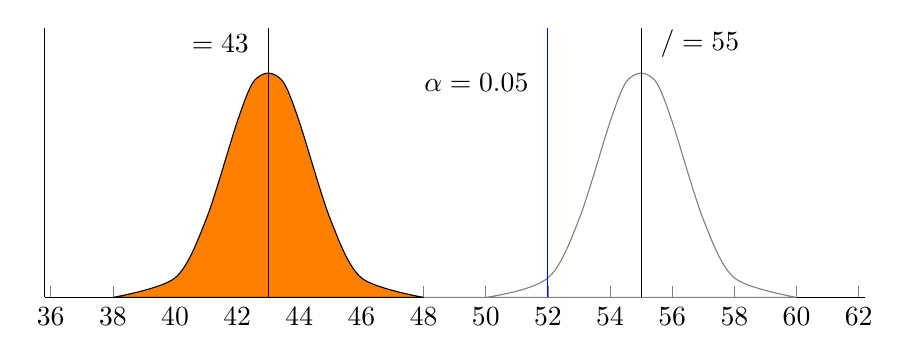
\begin{tikzpicture}
    \begin{axis}[
      axis lines*=left,
      ytick=\empty,
      height=5cm,
      width=12cm,
      enlarge y limits={value=0.2,upper},
      ]

      \addplot[smooth, color=gray, domain=45:65] 
        coordinates{
          (48, 0)
          (50, 0) (52, 0.5) (53, 2) (54, 4.5) (54.5, 5.5)
          (55, 5.75)
          (55.5, 5.5) (56, 4.5) (57, 2) (58, 0.5) (60, 0)} 
        \closedcycle;

      \draw (55, 0) -- (55, 10);
      \node at (55, 6.5) [label=right:{$\HypPopMean/ = 55$}] {};

      \addplot[smooth, fill=orange, domain=45:65] 
        coordinates{
          (38, 0) (40, 0.5) (41, 2) (42, 4.5) (42.5, 5.5)
          (43, 5.75)
          (43.5, 5.5) (44, 4.5) (45, 2) (46, 0.5) (48, 0)} 
        \closedcycle;

      \draw (43, 0) -- (43, 10);
      \node at (43, 6.5) [label=left:{$\populationmean = 43$}] {};

      \draw[color=blue] (52, 0) -- (52, 10);
      \node at (52, 5.5) [label=left:{$\alpha = 0.05$}] {};

    \end{axis}
  \end{tikzpicture}
\end{center}

\noindent
To say that this curve has a power test of 1 (or 100\%) is to say that this particular hypothesis test has a lot of power to distinguish these two curves. And indeed, that makes perfect sense. The test hypothesizes that the true population mean is at 55K, but if the actual population were at 43K, then any sample we could take would definitively be outside the hypothesized population, and so we will always correctly reject (rather than accept) the null hypothesis.


%%%%%%%%%%%%%%%%%%%%%%%%%%%%%%%%%%%%%%%%%
%%%%%%%%%%%%%%%%%%%%%%%%%%%%%%%%%%%%%%%%%
\section{A low power test value}

Now consider a case where the true population mean is very close to the hypothesized one, so that the two curves overlap a lot. For example, suppose the true population mean is 53. That is very close to the hypothesized mean, so the two will overlap considerably:

\begin{center}
  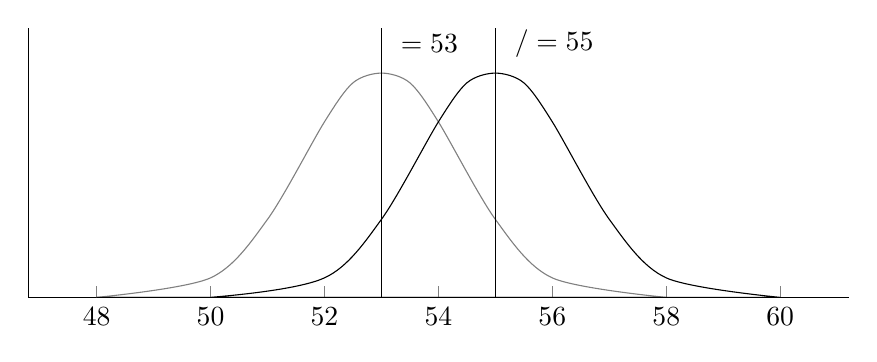
\begin{tikzpicture}
    \begin{axis}[
      axis lines*=left,
      ytick=\empty,
      height=5cm,
      width=12cm,
      enlarge y limits={value=0.2,upper},
      ]

      \addplot[smooth, color=gray, domain=45:65] 
        coordinates{
          (48, 0) (50, 0.5) (51, 2) (52, 4.5) (52.5, 5.5)
          (53, 5.75)
          (53.5, 5.5) (54, 4.5) (55, 2) (56, 0.5) (58, 0)} 
        \closedcycle;

      \addplot[smooth, color=black, domain=45:65] 
        coordinates{
          (48, 0)
          (50, 0) (52, 0.5) (53, 2) (54, 4.5) (54.5, 5.5)
          (55, 5.75)
          (55.5, 5.5) (56, 4.5) (57, 2) (58, 0.5) (60, 0)} 
        \closedcycle;

      \draw (55, 0) -- (55, 10);
      \node at (55, 6.5) [label=right:{$\HypPopMean/ = 55$}] {};

      \draw (53, 0) -- (53, 10);
      \node at (53, 6.5) [label=right:{$\populationmean = 53$}] {};

    \end{axis}
  \end{tikzpicture}
\end{center}

\noindent
Let's draw in the critical point, $\alpha$, at 0.05 again:

\begin{center}
  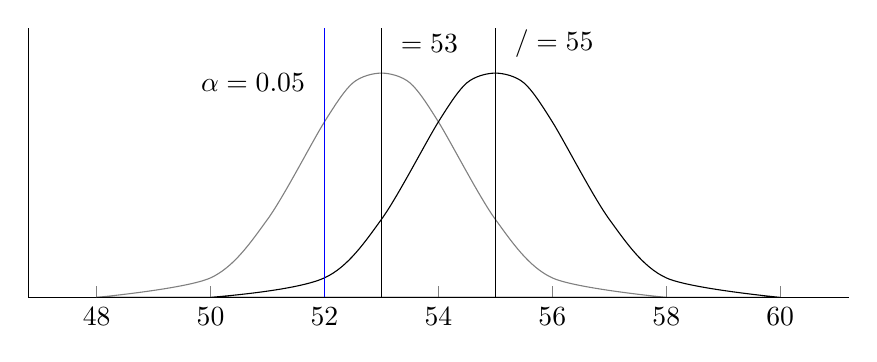
\begin{tikzpicture}
    \begin{axis}[
      axis lines*=left,
      ytick=\empty,
      height=5cm,
      width=12cm,
      enlarge y limits={value=0.2,upper},
      ]

      \addplot[smooth, color=gray, domain=45:65] 
        coordinates{
          (48, 0) (50, 0.5) (51, 2) (52, 4.5) (52.5, 5.5)
          (53, 5.75)
          (53.5, 5.5) (54, 4.5) (55, 2) (56, 0.5) (58, 0)} 
        \closedcycle;

      \addplot[smooth, color=black, domain=45:65] 
        coordinates{
          (48, 0)
          (50, 0) (52, 0.5) (53, 2) (54, 4.5) (54.5, 5.5)
          (55, 5.75)
          (55.5, 5.5) (56, 4.5) (57, 2) (58, 0.5) (60, 0)} 
        \closedcycle;

      \draw (55, 0) -- (55, 10);
      \node at (55, 6.5) [label=right:{$\HypPopMean/ = 55$}] {};

      \draw (53, 0) -- (53, 10);
      \node at (53, 6.5) [label=right:{$\populationmean = 53$}] {};

      \draw[color=blue] (52, 0) -- (52, 10);
      \node at (52, 5.5) [label=left:{$\alpha = 0.05$}] {};

    \end{axis}
  \end{tikzpicture}
\end{center}

\noindent
Let's now fill in the $\beta$ area:

\begin{center}
  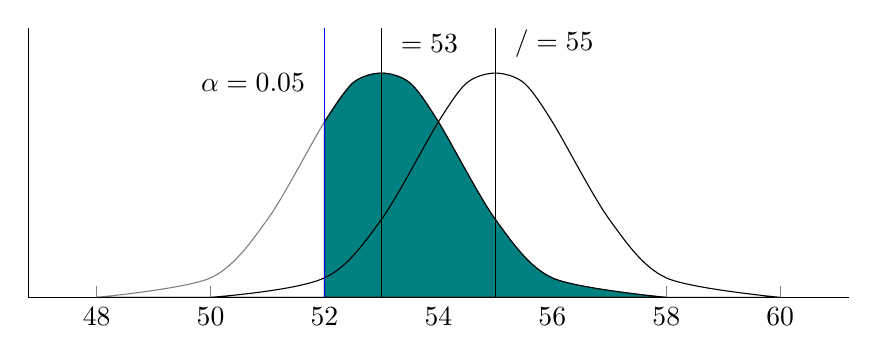
\begin{tikzpicture}
    \begin{axis}[
      axis lines*=left,
      ytick=\empty,
      height=5cm,
      width=12cm,
      enlarge y limits={value=0.2,upper},
      ]

      \addplot[smooth, color=gray, domain=45:65] 
        coordinates{
          (48, 0) (50, 0.5) (51, 2) (52, 4.5) (52.5, 5.5)
          (53, 5.75)
          (53.5, 5.5) (54, 4.5) (55, 2) (56, 0.5) (58, 0)} 
        \closedcycle;

      \addplot[smooth, fill=teal, domain=45:65] 
        coordinates{
          (52, 4.5) (52.5, 5.5)
          (53, 5.75)
          (53.5, 5.5) (54, 4.5) (55, 2) (56, 0.5) (58, 0)} 
        \closedcycle;

      \addplot[smooth, color=black, domain=45:65] 
        coordinates{
          (48, 0)
          (50, 0) (52, 0.5) (53, 2) (54, 4.5) (54.5, 5.5)
          (55, 5.75)
          (55.5, 5.5) (56, 4.5) (57, 2) (58, 0.5) (60, 0)} 
        \closedcycle;

      \draw (55, 0) -- (55, 10);
      \node at (55, 6.5) [label=right:{$\HypPopMean/ = 55$}] {};

      \draw (53, 0) -- (53, 10);
      \node at (53, 6.5) [label=right:{$\populationmean = 53$}] {};

      \draw[color=blue] (52, 0) -- (52, 10);
      \node at (52, 5.5) [label=left:{$\alpha = 0.05$}] {};

    \end{axis}
  \end{tikzpicture}
\end{center}

\noindent
Let's reflect on this case a little bit. If the true population mean is 53, then we can get a sample mean from anywhere inside of the curve centered around 53. We've highlighted the area that is to the right of $\alpha$ on that curve. If we get any sample mean that falls in the highlighted area, we will have a sample that we (as humans) cannot tell if it belongs to the true population mean or the hypothesized population mean. For example, suppose we take a sample, and that sample has a mean of 56.25:

\begin{center}
  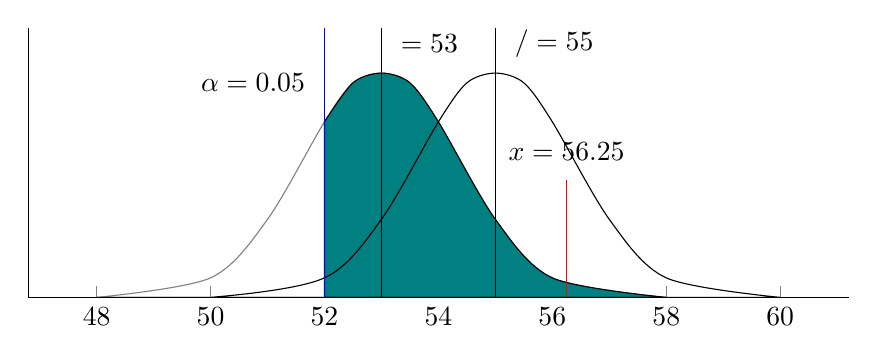
\begin{tikzpicture}
    \begin{axis}[
      axis lines*=left,
      ytick=\empty,
      height=5cm,
      width=12cm,
      enlarge y limits={value=0.2,upper},
      ]

      \addplot[smooth, color=gray, domain=45:65] 
        coordinates{
          (48, 0) (50, 0.5) (51, 2) (52, 4.5) (52.5, 5.5)
          (53, 5.75)
          (53.5, 5.5) (54, 4.5) (55, 2) (56, 0.5) (58, 0)} 
        \closedcycle;

      \addplot[smooth, fill=teal, domain=45:65] 
        coordinates{
          (52, 4.5) (52.5, 5.5)
          (53, 5.75)
          (53.5, 5.5) (54, 4.5) (55, 2) (56, 0.5) (58, 0)} 
        \closedcycle;

      \addplot[smooth, color=black, domain=45:65] 
        coordinates{
          (48, 0)
          (50, 0) (52, 0.5) (53, 2) (54, 4.5) (54.5, 5.5)
          (55, 5.75)
          (55.5, 5.5) (56, 4.5) (57, 2) (58, 0.5) (60, 0)} 
        \closedcycle;

      \draw (55, 0) -- (55, 10);
      \node at (55, 6.5) [label=right:{$\HypPopMean/ = 55$}] {};

      \draw (53, 0) -- (53, 10);
      \node at (53, 6.5) [label=right:{$\populationmean = 53$}] {};

      \draw[color=blue] (52, 0) -- (52, 10);
      \node at (52, 5.5) [label=left:{$\alpha = 0.05$}] {};
      
      \draw[color=red] (56.25, 0) -- (56.25, 3);
      \node at (56.25, 3) [label=above:{$\samplemean{x} = 56.25$}] {};

    \end{axis}
  \end{tikzpicture}
\end{center}

\noindent
As humans, we cannot tell if this sample comes from the hypothesized population, or the true one. So what should we do in this case? As always, we should follow our procedure. Since the sample mean is greater than $\alpha$, we will accept the null hypothesis. But we can see (as an all-seeing God or Oracle) that this is incorrect. We should not have accepted the null hypothesis, because the sample comes from a different population than the hypothesized one. It comes from the population centered at 53K.

Let's think about the power test value now. To see it, let's highlight it:

\begin{center}
  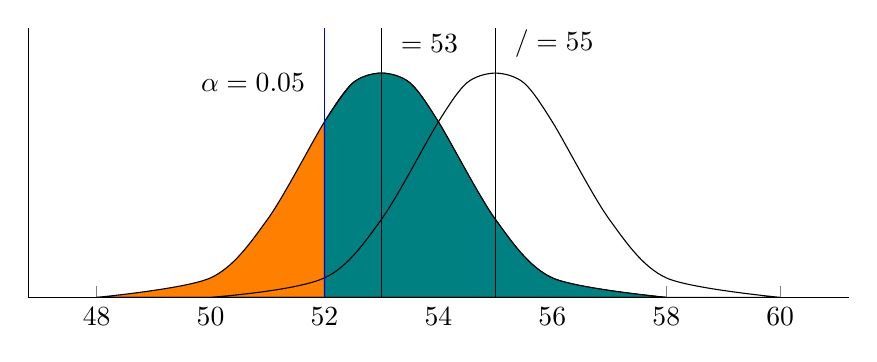
\begin{tikzpicture}
    \begin{axis}[
      axis lines*=left,
      ytick=\empty,
      height=5cm,
      width=12cm,
      enlarge y limits={value=0.2,upper},
      ]

      \addplot[smooth, fill=orange, domain=45:65] 
        coordinates{
          (48, 0) (50, 0.5) (51, 2) (52, 4.5) (52.5, 5.5)
          (53, 5.75)
          (53.5, 5.5) (54, 4.5) (55, 2) (56, 0.5) (58, 0)} 
        \closedcycle;

      \addplot[smooth, fill=teal, domain=45:65] 
        coordinates{
          (52, 4.5) (52.5, 5.5)
          (53, 5.75)
          (53.5, 5.5) (54, 4.5) (55, 2) (56, 0.5) (58, 0)} 
        \closedcycle;

      \addplot[smooth, color=black, domain=45:65] 
        coordinates{
          (48, 0)
          (50, 0) (52, 0.5) (53, 2) (54, 4.5) (54.5, 5.5)
          (55, 5.75)
          (55.5, 5.5) (56, 4.5) (57, 2) (58, 0.5) (60, 0)} 
        \closedcycle;

      \draw (55, 0) -- (55, 10);
      \node at (55, 6.5) [label=right:{$\HypPopMean/ = 55$}] {};

      \draw (53, 0) -- (53, 10);
      \node at (53, 6.5) [label=right:{$\populationmean = 53$}] {};

      \draw[color=blue] (52, 0) -- (52, 10);
      \node at (52, 5.5) [label=left:{$\alpha = 0.05$}] {};

    \end{axis}
  \end{tikzpicture}
\end{center}

\noindent
Suppose  we take a sample and the mean of that sample falls somewhere inside the power test area. For example, 51:

\begin{center}
  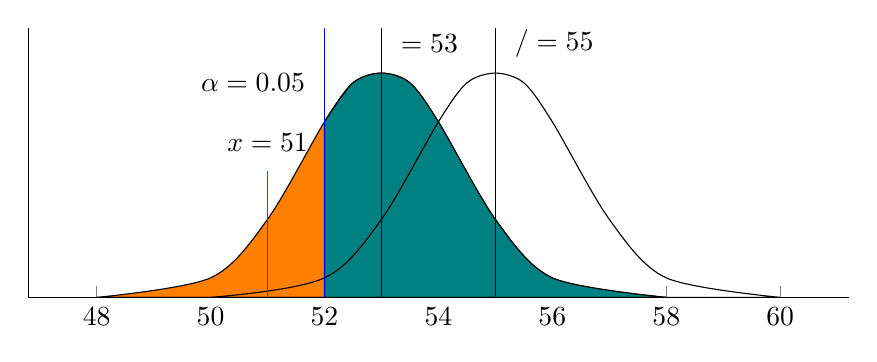
\begin{tikzpicture}
    \begin{axis}[
      axis lines*=left,
      ytick=\empty,
      height=5cm,
      width=12cm,
      enlarge y limits={value=0.2,upper},
      ]

      \addplot[smooth, fill=orange, domain=45:65] 
        coordinates{
          (48, 0) (50, 0.5) (51, 2) (52, 4.5) (52.5, 5.5)
          (53, 5.75)
          (53.5, 5.5) (54, 4.5) (55, 2) (56, 0.5) (58, 0)} 
        \closedcycle;

      \addplot[smooth, fill=teal, domain=45:65] 
        coordinates{
          (52, 4.5) (52.5, 5.5)
          (53, 5.75)
          (53.5, 5.5) (54, 4.5) (55, 2) (56, 0.5) (58, 0)} 
        \closedcycle;

      \addplot[smooth, color=black, domain=45:65] 
        coordinates{
          (48, 0)
          (50, 0) (52, 0.5) (53, 2) (54, 4.5) (54.5, 5.5)
          (55, 5.75)
          (55.5, 5.5) (56, 4.5) (57, 2) (58, 0.5) (60, 0)} 
        \closedcycle;

      \draw (55, 0) -- (55, 10);
      \node at (55, 6.5) [label=right:{$\HypPopMean/ = 55$}] {};

      \draw (53, 0) -- (53, 10);
      \node at (53, 6.5) [label=right:{$\populationmean = 53$}] {};

      \draw[color=blue] (52, 0) -- (52, 10);
      \node at (52, 5.5) [label=left:{$\alpha = 0.05$}] {};

      \draw[color=red] (51, 0) -- (51, 3.25);
      \node at (51, 3.25) [label=above:{$\samplemean{x} = 51$}] {};

    \end{axis}
  \end{tikzpicture}
\end{center}

\noindent
If we follow our procedure, what will we do? Since the sample mean falls below $\alpha$, we will reject the null hypothesis. Are we correct in doing so? Yes, because (as an all-seeing God or Oracle we can see that) the true population mean is centered at 53. 

And notice: the power test area tells us how good this particular test is at differentiating the two curves. In this case, there is not so much area in the power test region, which tells us that this test is not so good at differentiating the two curves. There is a lot of area in the $\beta$ region where we can mistakenly accept the null hypothesis. 

But this is not necessarily a bad thing. These curves are pretty close, after all, so it's not a terrible thing if we don't distinguish the hypothesized distribution from another one that is very, very close. Again, think of our original aim: we want to assume that the null hypothesis stands, unless we have strong evidence to overthrow it. And when the curves are really close, we're just not going to get strong evidence to overthrow the null hypothesis. As the curves get farther apart, of course, we do start getting stronger evidence.


%%%%%%%%%%%%%%%%%%%%%%%%%%%%%%%%%%%%%%%%%
%%%%%%%%%%%%%%%%%%%%%%%%%%%%%%%%%%%%%%%%%
\section{Conclusions}

From these examples, we can see the following:

\begin{itemize}

  \item The power test value goes up (and the $\beta$ value goes down) when the curves get farther apart, whereas the power test value goes down (and the $\beta$ value goes up) when the curves get closer together.

  \item As the curves get farther apart, the test gets better at distinguishing the curves (and hence the chance of making a Type II Error goes down), whereas as the curves get closer together, the test gets weaker at distinguishing the curves (and hence the chance of making a Type II Error goes up). 

  \item But having a high probability of a Type II Error simply means that we cannot distinguish the hypothesized population from one that is very close.

\end{itemize}

\end{document}
